\chapter{Arhitektura i dizajn sustava}
		

		\textnormal{ Arhitektura sustava ovog projekta može se podijeliti u tri dijela:}
	\begin{itemize}
		\item 	\textit{Baza podataka}
		\item 	\textit{Web aplikacija}
		\item 	\textit{Web poslužitelj}		
	\end{itemize}
\textnormal {\textbf{Web poslužitelj} osnova je rada web aplikacije. Njegova primarna zadaća je komunikacija klijenta s aplikacijom. Komunikacija se odvija preko HTTP (engl. Hyper Text Transfer Protocol) protokola. Poslužitelj je onaj koji pokreće web aplikaciju te joj prosljeđuje zahtjev. \textbf{Web preglednik} je program koji korisniku omogućuje pregled web stranica i multimedijalnih sadržaja vezanih uz njih. Korisnik i web aplikacija komuniciraju s web preglednikom. Korisnik preko \textbf{web aplikacije} šalje zahtjeve. Web aplikacija obrađuje zahtjeve te komunicira s bazom podataka. }
\bigbreak
\textnormal {Programski jezik koji smo odabrali za našu web aplikaciju jest C\#. Odabrali smo ga jer je većina današnjih web aplikacija napisana u C\#. Također, odlučili smo se na ASP.NET Core 3 radni okvir koji pruža mnogo funkcionalnosti. Koristimo i Vue.js radni okvir za JavaScript. Za razvojno okruženje odabrali smo Microsoft Visual Studio.}
\bigbreak
\textnormal{Arhitektura sustava temelji se na MVC (Model-View-Controller) konceptu. Taj je koncept podržan od ASP.NET Core 3 radnog okvira i olakšava razvoj web aplikacije zbog svojih gotovih predložaka. MVC koncept karakterističan je po tome što se pojedini dijelovi aplikacije mogu razvijati nezavisno, što uvelike olakšava testiranje, razvijanje te dodavanje novih mogućnosti u sustav. MVC koncept sadržava:}
\bigbreak
	\begin{itemize}
	\item 	\textbf{Model} - prima ulazne podatke od Controllera, predstavlja strukture podataka koje su dinamične i neovisne o korisničkom sučelju. Središnja je komponenta sustava jer izravno upravlja pravilima web aplikacije.
	\item 	\textbf{View} - prikaz podataka s mogućnosću različitih prikaza.
	\item 	\textbf{Controller}	- upravlja korisničkim zahtjevima te prima ulaze i prilagođava ih za prosljeđivanje Modelu ili Viewu, ovisno o potrebi.
\end{itemize}

	
		

		

				
		\section{Baza podataka}
			
			
		\textnormal{Za naš projekt odabrali smo relacijsku bazu podataka. Njezina osnovna jedinica je tablica definirana imenom i skupom atributa. Zadaća naše baze podataka je brza i jednostavna pohrana podataka, izmjena, brisanje i dohvat tih podataka. Baza podataka ove aplikacije sastoji se od sljedećih entiteta:}
		\smallbreak
			\begin{packed_item}
				\setlength\itemsep{0.01em}
			\item  Košarica
			\item  Korisnik
			\item  Narudžba
			\item Transakcija
			\item Artikl košarice
			\item Artikl narudžbe
			\item Artikl
			\item Artikl dostupnost
			\item Recenzija
			\item Utakmica
			\item Popust
			\item Slika
			\item Objava
			\item Igrač
		\end{packed_item}
		
		\pagebreak
		
			\subsection{Opis tablica}
			

				\textnormal{Tablica \textbf{Korisnik} opisuje svakog korisnika, klijenta, trenera, upravu ili administratora aplikacije. Sadrži atribute: korisničko ime, ime, prezime, e-mail, hash lozinke, razinu ovlasti, broj mobitela i datum registracije. Povezana je vezom \textit{One-to-Many} s entitetima Narudžba, Košarica i Recenzija preko korisničkog imena.}
				
				\begin{longtabu} to \textwidth {|X[8, l]|X[6, l]|X[20, l]|}
					
					\hline \multicolumn{3}{|c|}{\textbf{Korisnik}}	 \\[3pt] \hline
					\endfirsthead
					
					\hline \multicolumn{3}{|c|}{\textbf{Korisnik}}	 \\[3pt] \hline
					\endhead
					
					\hline 
					\endlastfoot
					
					\textbf{korisnicko\_ime}  & VARCHAR	&  jedinstveni identifikator korisnika	\\ \hline
					ime	& VARCHAR &   ime korisnika	\\ \hline 
					prezime & VARCHAR & prezime korisnika \\ \hline
					e-mail & VARCHAR & e-mail korisnika  \\ \hline 
					lozinka\_hash & VARCHAR	&  	hash lozinke	\\ \hline 
					razina\_ovlasti & INT & razina ovlasti korisnika \\ \hline
					broj\_mob & VARCHAR & broj mobitela korisnika \\ \hline 
					datum\_registracije	& TIMESTAMP & datum registracije korisnika   	\\ \hline 
					
					
				\end{longtabu}
			
			\textnormal{Tablica \textbf{Košarica} opisuje košarice koje se koriste u web shop-u. Sadrži atribute: ID, korisničko ime te datum kreiranja košarice. Povezana je vezom \textit{One-to-Many} s entitetom Artikl Košarice preko ID-a i \textit{Many-to-One} s entitetom Korisnik preko korisničkog imena. }
			
			\begin{longtabu} to \textwidth {|X[8, l]|X[6, l]|X[20, l]|}
				
				\hline \multicolumn{3}{|c|}{\textbf{Košarica}}	 \\[3pt] \hline
				\endfirsthead
				
				\hline \multicolumn{3}{|c|}{\textbf{Košarica }}	 \\[3pt] \hline
				\endhead
				
				\hline 
				\endlastfoot
				
				\textbf{ID} & INT	&  jedinstveni identifikator košarice	\\ \hline
				\textit{korisnicko\_ime} 	& VARCHAR &   ime korisnika koji koristi košaricu	\\ \hline 
				datum& TIMESTAMP & datum kreiranja košarice	\\ \hline 
				
			\end{longtabu}
		
		
		\textnormal{Tablica \textbf{Artikl Košarice} opisuje artikle košarice koje se koriste u web shop-u. Sadrži atribute: ID košarice, ID artikla, količinu artikla, veličinu artikla, kupovnu cijenu i kupovni popust. Povezana je vezom \textit{Many-to-One} s entitetima Artikl i Košarica preko ID artikla, odnosno ID košarice.}
		
		\begin{longtabu} to \textwidth {|X[8, l]|X[6, l]|X[20, l]|}
			
			\hline \multicolumn{3}{|c|}{\textbf{Artikl Košarice}}	 \\[3pt] \hline
			\endfirsthead
			
			\hline \multicolumn{3}{|c|}{\textbf{Artikl Košarice }}	 \\[3pt] \hline
			\endhead
			
			\hline 
			\endlastfoot
			
			\textbf{ID\_košarice} & INT	&  jedinstveni identifikator košarice	\\ \hline
			\textbf{ID\_artikla}	& int &  jedinstveni identifikator artikla	\\ \hline 
			kolicina & INT  & količina artikla \\ \hline 
			velicina & VARCHAR  & veličina artikla \\ \hline 
			kupovna\_cijena & DECIMAL  & kupovna cijena artikla \\ \hline 
			kupovni\_popust & INT  & kupovni popust artikla  \\ \hline 
			
		\end{longtabu}
		\textnormal{Tablica \textbf{Recenzija} opisuje recenzije ostavljene artiklu u web shop-u. Sadrži atribute: ID, ID artikla, datum, ocjena, komentar, korisničko ime i blokirano. Povezana je vezom \textit{Many-to-One} s entitima Artikl i Korisnik preko ID artikla, odnosno korisničkog imena. }
	
	\begin{longtabu} to \textwidth {|X[8, l]|X[6, l]|X[20, l]|}
		
		\hline \multicolumn{3}{|c|}{\textbf{Recenzija}}	 \\[3pt] \hline
		\endfirsthead
		
		\hline \multicolumn{3}{|c|}{\textbf{Recenzija}}	 \\[3pt] \hline
		\endhead
		
		\hline 
		\endlastfoot
		
		\textbf{ID} & INT	&  jedinstveni identifikator recenzije	\\ \hline
		\textit{ID\_artikla}	& INT &  jedinstveni identifikator artikla	\\ \hline 
		datum & TIMESTAMP  & datum dodavanja recenzije \\ \hline 
		ocjena & INT  & ocjena artikla \\ \hline 
		komentar & VARCHAR  & komentar recenzije \\ \hline 
		korisnicko\_ime & INT  & korisničko ime korisnika koji ostavlja recenziju  \\ \hline 
		blokirano & BOOLEAN  & dozvoljena ili blokirana recenzija \\ \hline 
		
	\end{longtabu}

	\textnormal{Tablica \textbf{Utakmica} opisuje utakmice kluba. Sadrži atribute: ID, datum, tim domacin, tim gost, mjesto, dvorana i drzava. }

\begin{longtabu} to \textwidth {|X[8, l]|X[6, l]|X[20, l]|}
	
	\hline \multicolumn{3}{|c|}{\textbf{Utakmica}}	 \\[3pt] \hline
	\endfirsthead
	
	\hline \multicolumn{3}{|c|}{\textbf{Utakmica}}	 \\[3pt] \hline
	\endhead
	
	\hline 
	\endlastfoot
	
	\textbf{ID} & INT	&  jedinstveni identifikator utakmice	\\ \hline
	datum & TIMESTAMP &  jedinstveni identifikator artikla	\\ \hline 
	tim\_domacin & VARCHAR  & tim domaćin utakmice \\ \hline 
	tim\_gost & VARCHAR  & tim gost utakmice  \\ \hline 
	mjesto & VARCHAR  & mjesto održavanja utakmice \\ \hline 
	dvorana & VARCHAR  & dvorana održavanja utakmice \\ \hline 
	drzava & VARCHAR  & država održavanja utakmice \\ \hline 
	
\end{longtabu}

\textnormal{Tablica \textbf{Popust} opisuje popuste na artikl dodane na web shop. Sadrži atribute: ID, ID artikla, datum, datum pocetka, datum kraja i postotak popusta. Entitet je povezan vezom \textit{Many-to-One} s entitetom Artikl preko ID artikla.}

\begin{longtabu} to \textwidth {|X[8, l]|X[6, l]|X[20, l]|}
	
	\hline \multicolumn{3}{|c|}{\textbf{Popust}}	 \\[3pt] \hline
	\endfirsthead
	
	\hline \multicolumn{3}{|c|}{\textbf{Popust}}	 \\[3pt] \hline
	\endhead
	
	\hline 
	\endlastfoot
	
	\textbf{ID} & INT	&  jedinstveni identifikator popusta	\\ \hline
	\textit{ID\_artikla} & INT &  jedinstveni identifikator artikla	\\ \hline 
	datum & TIMESTAMP  & datum stvaranja popusta \\ \hline 
	datum\_pocetka & TIMESTAMP  & datum početka popusta  \\ \hline 
	datum\_kraja & TIMESTAMP  & datum završetka popusta \\ \hline 
	postotak & INT  & postotak popusta \\ \hline 
	
\end{longtabu}

\textnormal{Tablica \textbf{Slika} opisuje slike dodane na web stranicu. Sadrži atribute: ID, path, datum. Entitet je povezan vezom \textit{One-to-Many} s entitetima Artikl, Objava i Igrač preko ID slike.}

\begin{longtabu} to \textwidth {|X[8, l]|X[6, l]|X[20, l]|}
	
	\hline \multicolumn{3}{|c|}{\textbf{Slika}}	 \\[3pt] \hline
	\endfirsthead
	
	\hline \multicolumn{3}{|c|}{\textbf{Slika}}	 \\[3pt] \hline
	\endhead
	
	\hline 
	\endlastfoot
	
	\textbf{ID} & INT	&  jedinstveni identifikator slike	\\ \hline
     path & VARCHAR  &  put do slike	\\ \hline 
	datum & TIMESTAMP  & datum dodavanja slike \\ \hline 
\end{longtabu}

\textnormal{Tablica \textbf{Artikl} opisuje artikle dodane na web shop. Sadrži atribute: ID, datum dodavanja, datum posljednje izmjene, tip, cijenu, naziv, opis, ID slike. Entitet je povezan vezom \textit{One-to-Many} s entitetima Artikl Dostupnost, Popust, Artikl Narudžbe, Recenzija te Artikl Košarice preko ID artikla i vezom \textit{Many-to-One} s entitetom Slika preko ID slike.}

\begin{longtabu} to \textwidth {|X[8, l]|X[6, l]|X[20, l]|}
	
	\hline \multicolumn{3}{|c|}{\textbf{Artikl}}	 \\[3pt] \hline
	\endfirsthead
	
	\hline \multicolumn{3}{|c|}{\textbf{Artikl}}	 \\[3pt] \hline
	\endhead
	
	\hline 
	\endlastfoot
	
	\textbf{ID} & INT	&  jedinstveni identifikator artikla	\\ \hline
	datum\_dodavanja & TIMESTAMP  & datum dodavanja artikla \\ \hline 
	datum\_izmjene & TIMESTAMP  & datum posljednje izmjene slike \\ \hline 
	tip & VARCHAR  & tip artikla \\ \hline 
	cijena & INT  & cijena artikla \\ \hline 
	naziv  & VARCHAR  & naziv artikla \\ \hline 
	opis & VARCHAR  & opis artikla \\ \hline 
	\textit{ID\_slike} & INT  & jedinstveni identifikator slike  \\ \hline 
	 
\end{longtabu}
\textnormal{Tablica \textbf{Narudžba} opisuje narudžbe artikala aplikacije. Sadrži atribute: ID, ID transakcije, korisničko ime, datum, zaprimljenost, adresa, mjesto, poštanski broj. Entitet je povezan vezom \textit{One-to-Many} s entitetima Artikl Narudžbe i Transakcija preko ID narudžbe i vezom \textit{Many-to-One} s entitetom Korisnik preko korisničkog imena.}

\begin{longtabu} to \textwidth {|X[8, l]|X[6, l]|X[20, l]|}
	
	\hline \multicolumn{3}{|c|}{\textbf{Narudžba}}	 \\[3pt] \hline
	\endfirsthead
	
	\hline \multicolumn{3}{|c|}{\textbf{Narudžba}}	 \\[3pt] \hline
	\endhead
	
	\hline 
	\endlastfoot
	
	\textbf{ID} & INT	&  jedinstveni identifikator narudžbe	\\ \hline
	\textit{ID\_transakcije} & INT  & jedinstveni identifikator transakcije \\ \hline 
	\textit{korisnicko\_ime} & VARCHAR  & korisničko ime korisnika koji naručuje \\ \hline 
	datum & TIMESTAMP  & datum formiranja narudžbe\\ \hline 
	zaprimljenost & BOOLEAN  & oznaka zaprimljenosti narudžbe \\ \hline 
	adresa  & VARCHAR  & adresa korisnika koji naručuje \\ \hline 
	mjesto & VARCHAR  & mjesto korisnika koji naručuje\\ \hline 
	postanski\_broj & INT  & poštanski broj korisnika koji naručuje\\ \hline 
	
\end{longtabu}

\textnormal{Tablica \textbf{Objava} opisuje sadržaje objavljene na stranici. Sadrži atribute: ID, sadržaj, ID slike, datum objave, datum izmjene, vrsta objave, datum pocetka i datum isteka. Entitet je povezan  vezom \textit{Many-to-One} s entitetom Slika preko ID slike.}

\begin{longtabu} to \textwidth {|X[8, l]|X[6, l]|X[20, l]|}
	
	\hline \multicolumn{3}{|c|}{\textbf{Objava}}	 \\[3pt] \hline
	\endfirsthead
	
	\hline \multicolumn{3}{|c|}{\textbf{Objava}}	 \\[3pt] \hline
	\endhead
	
	\hline 
	\endlastfoot
	
	\textbf{ID} & INT	&  jedinstveni identifikator objave	\\ \hline
	 sadržaj & VARCHAR  & sadržaj objave \\ \hline 
	\textit{ID\_slike} & ID  & jedinstveni identifikator slike  \\ \hline 
	datum\_objave & TIMESTAMP  & datum postavljanja objave \\ \hline 
	datum\_izmjene & TIMESTAMP  & datum posljednje izmjene objave \\ \hline
	vrsta\_objave & VARCHAR  & vrsta objave \\ \hline 
	datum\_pocetka & TIMESTAMP  & datum početka objave \\ \hline
	datum\_isteka & TIMESTAMP  & datum isteka objave \\ \hline
	
\end{longtabu}
\textnormal{Tablica \textbf{Transakcija} opisuje sve obavljane transakcije. Sadrži atribute: ID, datum, iznos, kartica. Entitet je povezan  vezom \textit{One-to-Many} s entitetom Narudžba preko ID transakcije.}

\begin{longtabu} to \textwidth {|X[8, l]|X[6, l]|X[20, l]|}
	
	\hline \multicolumn{3}{|c|}{\textbf{Transakcija}}	 \\[3pt] \hline
	\endfirsthead
	
	\hline \multicolumn{3}{|c|}{\textbf{Transakcija}}	 \\[3pt] \hline
	\endhead
	
	\hline 
	\endlastfoot
	
	\textbf{ID} & INT	&  jedinstveni identifikator transakcije	\\ \hline
	datum & TIMESTAMP  & datum obavljanja transakcije  \\ \hline 
	iznos & DECIMAL  & iznos transakcije \\ \hline
	kartica & VARCHAR  & kartica transakcije  \\ \hline 
	
\end{longtabu}

\textnormal{Tablica \textbf{Artikl dostupnost} opisuje dostupnost artikala. Sadrži atribute: ID artikla, veličina i količina. Entitet je povezan  vezom \textit{Many-to-One} s entitetom Artikla preko ID artikla.}

\begin{longtabu} to \textwidth {|X[8, l]|X[6, l]|X[20, l]|}
	
	\hline \multicolumn{3}{|c|}{\textbf{Artikl dostupnost}}	 \\[3pt] \hline
	\endfirsthead
	
	\hline \multicolumn{3}{|c|}{\textbf{Artikl dostupnost}}	 \\[3pt] \hline
	\endhead
	
	\hline 
	\endlastfoot
	
	\textbf{ID\_artikla} & INT	&  jedinstveni identifikator artikla	\\ \hline
	količina & INT  & količina artikla  \\ \hline 
	veličina & VARCHAR  & veličina artikla \\ \hline
	
\end{longtabu}

\textnormal{Tablica \textbf{Artikl narudžbe} opisuje sve artikle narudžbe. Sadrži atribute: ID narudžbe, ID artikla, količina, veličina, kupovna cijena i kupovni popust. Entitet je povezan  vezom \textit{Many-to-One} s entitetima Narudžba preko ID narudžbe i Artikl preko ID artikla.}

\begin{longtabu} to \textwidth {|X[8, l]|X[6, l]|X[20, l]|}
	
	\hline \multicolumn{3}{|c|}{\textbf{Artikl narudžbe}}	 \\[3pt] \hline
	\endfirsthead
	
	\hline \multicolumn{3}{|c|}{\textbf{Artikl narudžbe}}	 \\[3pt] \hline
	\endhead
	
	\hline 
	\endlastfoot
	
	\textbf{ID\_narudzbe} & INT	&  jedinstveni identifikator narudžbe	\\ \hline
	\textbf{ID\_artikla} & INT	&  jedinstveni identifikator artikla	\\ \hline
	količina & INT  & količina artikla  \\ \hline 
	veličina & VARCHAR  & veličina artikla \\ \hline
	kupovna\_cijena & DECIMAL  & kupovna cijena  \\ \hline 
	kupovni\_popust & INT  & kupovni popust \\ \hline
	
\end{longtabu}

\textnormal{Tablica \textbf{Igrač} opisuje sve igrače. Sadrži atribute: ID, datum dodavanja, datum posljednje izmjene, ime, prezime, ID slike, datum rođenja i pozicija. Entitet je povezan vezom \textit{Many-to-One} s entitetom Slika.}

\begin{longtabu} to \textwidth {|X[8, l]|X[6, l]|X[20, l]|}
	
	\hline \multicolumn{3}{|c|}{\textbf{Igrač}}	 \\[3pt] \hline
	\endfirsthead
	
	\hline \multicolumn{3}{|c|}{\textbf{Igrač}}	 \\[3pt] \hline
	\endhead
	
	\hline 
	\endlastfoot
	
	\textbf{ID\_narudzbe} & INT	&  jedinstveni identifikator igrača	\\ \hline
	datum\_dodavanja & TIMESTAMP  & datum dodavanja igrača \\ \hline 
	datum\_izmjene & TIMESTAMP  & datum izmjene igrača \\ \hline 
	ime & VARCHAR  & ime igrača \\ \hline
	prezime & VARCHAR  & prezime igrača \\ \hline
	ID\_slike & INT  & jedinstveni identifikator slike igrača \\ \hline
	datum\_rodenja & DATE  & datum rođenja igrača \\ \hline 
	pozicija & VARCHAR  & pozicija igrača \\ \hline
	
	
\end{longtabu}
	

	
	
		
		
			
			
			\subsection{Dijagram baze podataka}
					\begin{figure}[H]
					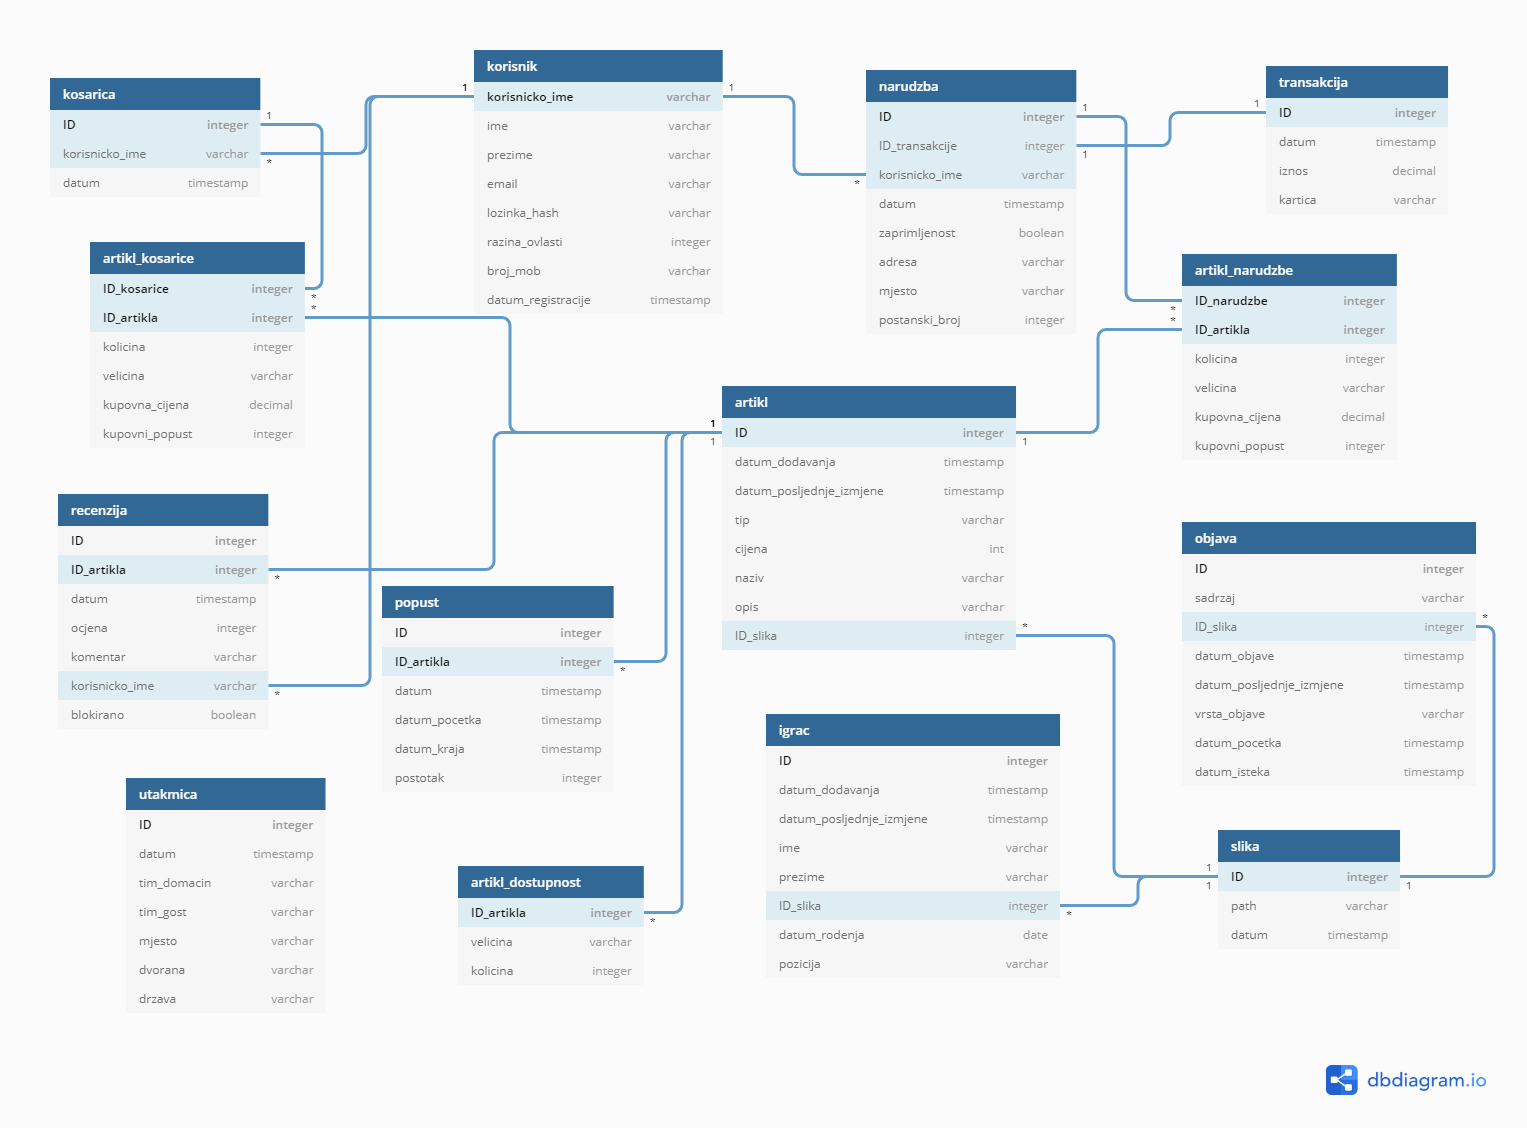
\includegraphics[width=\linewidth]{dijagrami/bazapodataka.png}
					\centering
					\caption{Dijagram baze podataka}
					\label{fig:DatabaseDiagram}
				\end{figure}
			
			\eject
			
			
		\section{Dijagram razreda}
		
			\textnormal{Na slikama 4.2 i 4.3 su prikazani razredi koji pripadaju backend dijelu MVC arhitekture. Razredi prikazani na slici 4.2 nasljeđuju Controller razred. Razredi su podijeljeni prema pravu pristupa metodama određenih aktora. Iz naziva i tipova atributa u razredima može se zaključiti vrsta ovisnosti medu različitim razredima.}\\
			
			\begin{figure}[H]
				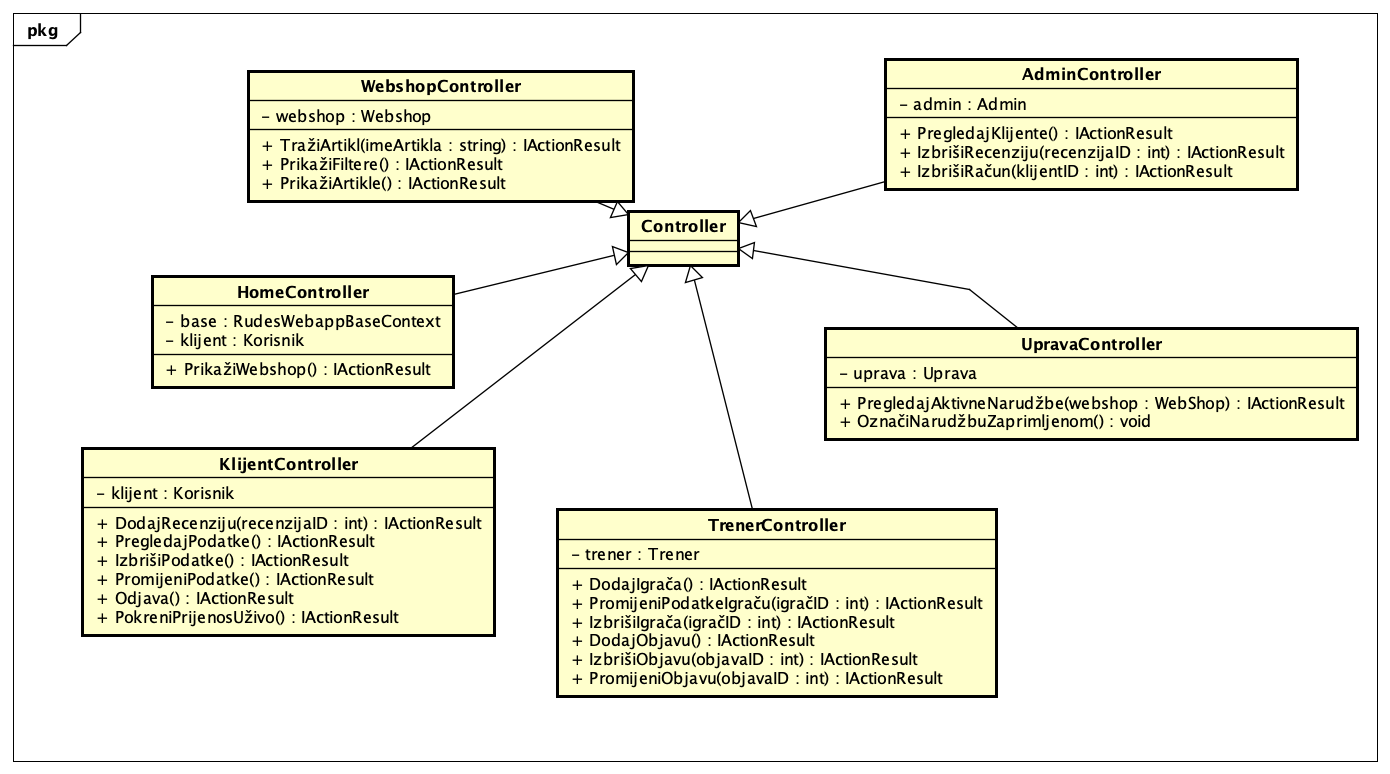
\includegraphics[width=\linewidth]{dijagrami/DijagramRazredaController.png}
				\centering
				\caption{Dijagram razreda - dio Controllers}
				\label{fig:ClassDiagram1}
			\end{figure}
		
			\textnormal{Model razredi na slici 4.3 preslikavaju strukturu baze podataka u aplikaciji. Implementirane metode direktno komuniciraju s bazom podataka te vraćaju tražene podatke. Razred Objava predstavlja objavu bilo koje vrste koja se prikazuje na stranici. Razred Igrač predstavlja igrače kluba kojima se mogu mijenjati podaci. Razred Slika predstavlja sve slike iz objava ili igrača. Razred Utakmica predstavlja utakmice koje klub igra. Nadalje, razredi Artikl, Popust, Artikl Dostupnost i Artikl Košarica predstavljaju artikle, odnosno popuste, dostupnost artikala i artikle stavljene u košaricu web shop-a kluba. Također, razredi Narudžba i Narudžba Artikl i Košarica također su vezani uz web shop. Narudžba predstavlja sve narudžbe korisnika, Narudžba Artikl sve artikle jedne narudžbe, dok razred Košarica predstavlja košaricu web shop-a. Razred Transakcija su sve transakcije koje se obavljaju u web shop-u između klijenata kluba i banke. Razred Recenzija predstavlja recenzije proizvoda u web shopu koje razred Korisnik može ostaviti. Razred Korisnik predstavlja korisnike sustava koji se mogu registrirati i prijaviti u sustav.}\\
		
		\begin{figure}[H]
			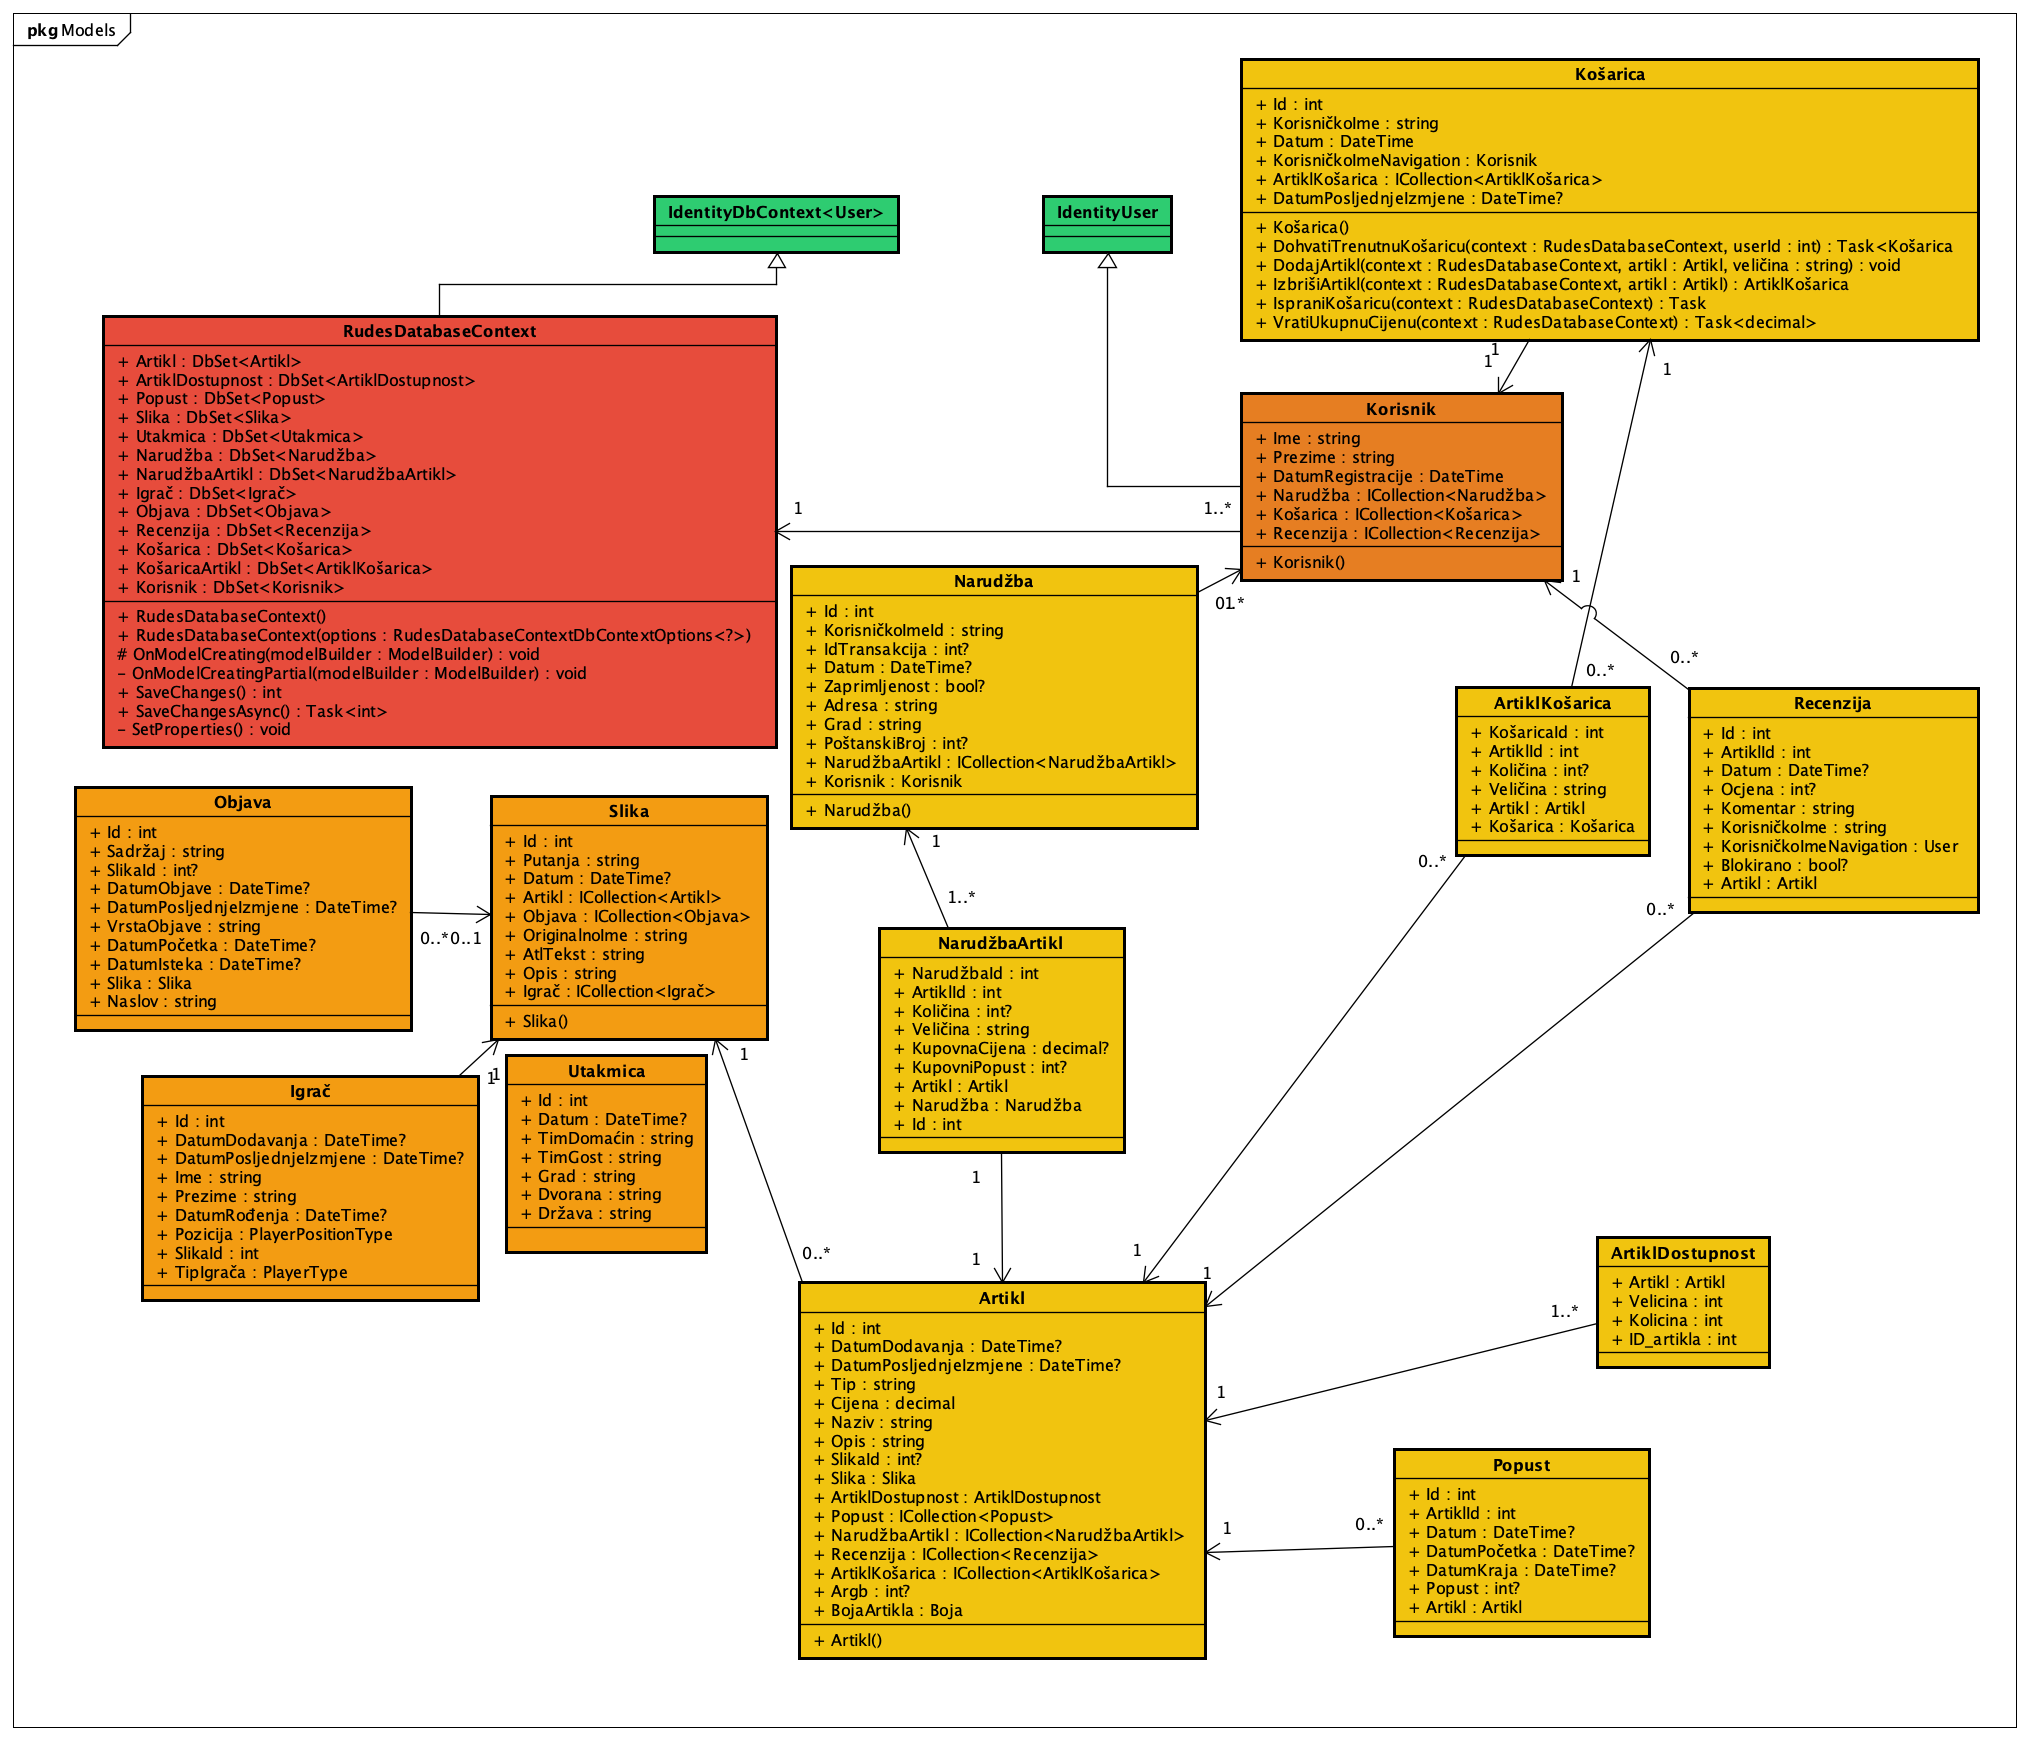
\includegraphics[width=\linewidth]{dijagrami/DijagramRazredaModels.png}
			\centering
			\caption{Dijagram razreda - dio Models}
			\label{fig:ClassDiagram1}
		\end{figure}
			
		%	\textbf{\textit{dio 1. revizije}}\\
			
		%	\textit{Prilikom prve predaje projekta, potrebno je priložiti potpuno razrađen dijagram razreda vezan uz \textbf{generičku funkcionalnost} sustava. Ostale funkcionalnosti trebaju biti idejno razrađene u dijagramu sa sljedećim komponentama: nazivi razreda, nazivi metoda i vrste pristupa metodama (npr. javni, zaštićeni), nazivi atributa razreda, veze i odnosi između razreda.}\\
			
		%	\textbf{\textit{dio 2. revizije}}\\			
			
		%	\textit{Prilikom druge predaje projekta dijagram razreda i opisi moraju odgovarati stvarnom stanju implementacije}
			
			
			
			\eject
		
		% \section{Dijagram stanja}
			
			
		% 	\textbf{\textit{dio 2. revizije}}\\
			
		% 	\textit{Potrebno je priložiti dijagram stanja i opisati ga. Dovoljan je jedan dijagram stanja koji prikazuje \textbf{značajan dio funkcionalnosti} sustava. Na primjer, stanja korisničkog sučelja i tijek korištenja neke ključne funkcionalnosti jesu značajan dio sustava, a registracija i prijava nisu. }
			
			
		% 	\eject 
		
		% \section{Dijagram aktivnosti}
			
		% 	\textbf{\textit{dio 2. revizije}}\\
			
		% 	 \textit{Potrebno je priložiti dijagram aktivnosti s pripadajućim opisom. Dijagram aktivnosti treba prikazivati značajan dio sustava.}
			
		% 	\eject
		% \section{Dijagram komponenti}
		
		% 	\textbf{\textit{dio 2. revizije}}\\
		
		% 	 \textit{Potrebno je priložiti dijagram komponenti s pripadajućim opisom. Dijagram komponenti treba prikazivati strukturu cijele aplikacije.}